%%%%%%%%%%%%%%%%%%%%%%%%%%%%%%%%%%%%%%%%%
% Beamer Presentation
% LaTeX Template
% Version 2.0 (March 8, 2022)
%
% This template originates from:
% https://www.LaTeXTemplates.com
%
% Author:
% Vel (vel@latextemplates.com)
%
% License:
% CC BY-NC-SA 4.0 (https://creativecommons.org/licenses/by-nc-sa/4.0/)
%
%%%%%%%%%%%%%%%%%%%%%%%%%%%%%%%%%%%%%%%%%

%----------------------------------------------------------------------------------------
%	PACKAGES AND OTHER DOCUMENT CONFIGURATIONS
%----------------------------------------------------------------------------------------

\documentclass[
	11pt, % Set the default font size, options include: 8pt, 9pt, 10pt, 11pt, 12pt, 14pt, 17pt, 20pt
	%t, % Uncomment to vertically align all slide content to the top of the slide, rather than the default centered
	%aspectratio=169, % Uncomment to set the aspect ratio to a 16:9 ratio which matches the aspect ratio of 1080p and 4K screens and projectors
]{beamer}

\graphicspath{{rplots/}{./}} % Specifies where to look for included images (trailing slash required)

\usepackage{booktabs, amsmath, amsfonts} % Allows the use of \toprule, \midrule and \bottomrule for better rules in tables


%----------------------------------------------------------------------------------------
%	SELECT LAYOUT THEME
%----------------------------------------------------------------------------------------

% Beamer comes with a number of default layout themes which change the colors and layouts of slides. Below is a list of all themes available, uncomment each in turn to see what they look like.

%\usetheme{default}
%\usetheme{AnnArbor}
%\usetheme{Antibes}
%\usetheme{Bergen}
%\usetheme{Berkeley}
%\usetheme{Berlin}
%\usetheme{Boadilla}
\usetheme{CambridgeUS}
%\usetheme{Copenhagen}
%\usetheme{Darmstadt}
%\usetheme{Dresden}
%\usetheme{Frankfurt}
%\usetheme{Goettingen}
%\usetheme{Hannover}
%\usetheme{Ilmenau}
%\usetheme{JuanLesPins}
%\usetheme{Luebeck}
%\usetheme{Madrid}
%\usetheme{Malmoe}
%\usetheme{Marburg}
%\usetheme{Montpellier}
%\usetheme{PaloAlto}
%\usetheme{Pittsburgh}
%\usetheme{Rochester}
%\usetheme{Singapore}
%\usetheme{Szeged}
%\usetheme{Warsaw}

%----------------------------------------------------------------------------------------
%	SELECT COLOR THEME
%----------------------------------------------------------------------------------------

% Beamer comes with a number of color themes that can be applied to any layout theme to change its colors. Uncomment each of these in turn to see how they change the colors of your selected layout theme.

%\usecolortheme{albatross}
%\usecolortheme{beaver}
%\usecolortheme{beetle}
%\usecolortheme{crane}
%\usecolortheme{dolphin}
%\usecolortheme{dove}
%\usecolortheme{fly}
%\usecolortheme{lily}
\usecolortheme{spruce}
%\usecolortheme{monarca}
%\usecolortheme{seagull}
%\usecolortheme{seahorse}
%\usecolortheme{whale}
%\usecolortheme{wolverine}

%----------------------------------------------------------------------------------------
%	SELECT FONT THEME & FONTS
%----------------------------------------------------------------------------------------

% Beamer comes with several font themes to easily change the fonts used in various parts of the presentation. Review the comments beside each one to decide if you would like to use it. Note that additional options can be specified for several of these font themes, consult the beamer documentation for more information.

\usefonttheme{default} % Typeset using the default sans serif font
%\usefonttheme{serif} % Typeset using the default serif font (make sure a sans font isn't being set as the default font if you use this option!)
%\usefonttheme{structurebold} % Typeset important structure text (titles, headlines, footlines, sidebar, etc) in bold
%\usefonttheme{structureitalicserif} % Typeset important structure text (titles, headlines, footlines, sidebar, etc) in italic serif
%\usefonttheme{structuresmallcapsserif} % Typeset important structure text (titles, headlines, footlines, sidebar, etc) in small caps serif

%------------------------------------------------

%\usepackage{mathptmx} % Use the Times font for serif text
\usepackage{palatino} % Use the Palatino font for serif text

\usepackage{natbib}
%\usepackage{helvet} % Use the Helvetica font for sans serif text
\usepackage[default]{opensans} % Use the Open Sans font for sans serif text
%\usepackage[default]{FiraSans} % Use the Fira Sans font for sans serif text
%\usepackage[default]{lato} % Use the Lato font for sans serif text

%----------------------------------------------------------------------------------------
%	SELECT INNER THEME
%----------------------------------------------------------------------------------------

% Inner themes change the styling of internal slide elements, for example: bullet points, blocks, bibliography entries, title pages, theorems, etc. Uncomment each theme in turn to see what changes it makes to your presentation.

%\useinnertheme{default}
\useinnertheme{circles}
%\useinnertheme{rectangles}
%\useinnertheme{rounded}
%\useinnertheme{inmargin}

%----------------------------------------------------------------------------------------
%	SELECT OUTER THEME
%----------------------------------------------------------------------------------------

% Outer themes change the overall layout of slides, such as: header and footer lines, sidebars and slide titles. Uncomment each theme in turn to see what changes it makes to your presentation.

%\useoutertheme{default}
%\useoutertheme{infolines}
%\useoutertheme{miniframes}
%\useoutertheme{smoothbars}
%\useoutertheme{sidebar}
%\useoutertheme{split}
%\useoutertheme{shadow}
%\useoutertheme{tree}
%\useoutertheme{smoothtree}

%\setbeamertemplate{footline} % Uncomment this line to remove the footer line in all slides
%\setbeamertemplate{footline}[page number] % Uncomment this line to replace the footer line in all slides with a simple slide count

%\setbeamertemplate{navigation symbols}{} % Uncomment this line to remove the navigation symbols from the bottom of all slides

%----------------------------------------------------------------------------------------
%	PRESENTATION INFORMATION
%----------------------------------------------------------------------------------------

\title[Statistical Project]{How do mental health medications impact the Body Mass Index?} % The short title in the optional parameter appears at the bottom of every slide, the full title in the main parameter is only on the title page


\author[Group 090]{Group 090} % Presenter name(s), the optional parameter can contain a shortened version to appear on the bottom of every slide, while the main parameter will appear on the title slide

\institute[EC124]{EC124 \\ \bigskip
\today}% Your institution, the optional parameter can be used for the institution shorthand and will appear on the bottom of every slide after author names, while the required parameter is used on the title slide and can include your email address or additional information on separate lines

\date[\today]{} % Presentation date or conference/meeting name, the optional parameter can contain a shortened version to appear on the bottom of every slide, while the required parameter value is output to the title slide

%----------------------------------------------------------------------------------------

\begin{document}

%----------------------------------------------------------------------------------------
%	TITLE SLIDE
%----------------------------------------------------------------------------------------

\begin{frame}
	\titlepage % Output the title slide, automatically created using the text entered in the PRESENTATION INFORMATION block above
\end{frame}

%----------------------------------------------------------------------------------------
%	TABLE OF CONTENTS SLIDE
%----------------------------------------------------------------------------------------

% The table of contents outputs the sections and subsections that appear in your presentation, specified with the standard \section and \subsection commands. You may either display all sections and subsections on one slide with \tableofcontents, or display each section at a time on subsequent slides with \tableofcontents[pausesections]. The latter is useful if you want to step through each section and mention what you will discuss.

\begin{frame}
	\frametitle{Presentation Overview} % Slide title, remove this command for no title
	
	\tableofcontents % Output the table of contents (all sections on one slide)
	%\tableofcontents[pausesections] % Output the table of contents (break sections up across separate slides)
\end{frame}

%----------------------------------------------------------------------------------------
%	PRESENTATION BODY SLIDES
%----------------------------------------------------------------------------------------

\section{Introduction} % Sections are added in order to organize your presentation into discrete blocks, all sections and subsections are automatically output to the table of contents as an overview of the talk but NOT output in the presentation as separate slides

%------------------------------------------------


\begin{frame} \subsection{Reasoning}
	\frametitle{Reasoning}
        \begin{itemize}
		\item 
                Mental health medication causes weight gain \citep{mazereel2020}.
		\begin{itemize}
			\item Hormonal imbalances
			\item Increased appetite
                \item Lowered physical activity
		\end{itemize}
  \end{itemize}

    \begin{itemize}
		\item 
                Literature is inconsistent when analysing magnitude of difference.
                \begin{itemize}
			\item Biological sex \citep{ALBERICH2019112506, Gates2016}
			\item Type of medication
   \citep{alonso, Vanina2002,mahli}
		\end{itemize}
  
	   \item We want to verify if these relationships still hold in England: 2019 Health Survey for England.
        \begin{itemize}
			\item Latest publicly available iteration before COVID-19
	   \end{itemize}
    \end{itemize}
 
 \end{frame}

%------------------------------------------------


%------------------------------------------------




%------------------------------------------------




\begin{frame}
	\frametitle{Dataset}
	%\framesubtitle{} % Optional subtitle
	
	\begin{itemize}
		\item \subsection{Dataset} \textbf{Dataset: }Health Survey for England 2019 [NS] (Adults aged 16+)
		\item \textbf{Number of observations: 10299}, of which 
		\begin{itemize}
			\item 8,205 adults (aged 16 and over) 
			\item 2,095 children (aged 0 to 15)
		\end{itemize}
	\item \textbf{After filtration, observations: 4358}, of which 
		\begin{itemize}
			\item 2437 female 
                \begin{itemize}
                    \item 388 Med Takers
                \end{itemize}
			\item 1921 male 
                \begin{itemize}
                    \item 163 Med Takers
                \end{itemize}
		\end{itemize}
  		\begin{itemize}
			\item 14 prescribed only antipsychotics 
			\item 16 prescribed only hypnotics
            \item 471 prescribed only antidepressants
		\end{itemize}
	\end{itemize}
 
\end{frame}

\begin{frame}
	\frametitle{Background} \subsection{Motivations} % Slide title, remove this command for no title
 Why this study was of particular interest to us:	
    \begin{itemize}
        \item With more openness in today's world about mental health diseases, the effects of taking medicines needs to be studied
        \item Obesity is associated with increased mortality, is placing a significant burden on healthcare systems globally
        \item With some literature linking the 2, existing studies have been inconclusive, where studies offer conflicting and unclear results
    \end{itemize}
\end{frame}



\begin{frame}{Filtered BMI Distribution} 
	\begin{figure}
		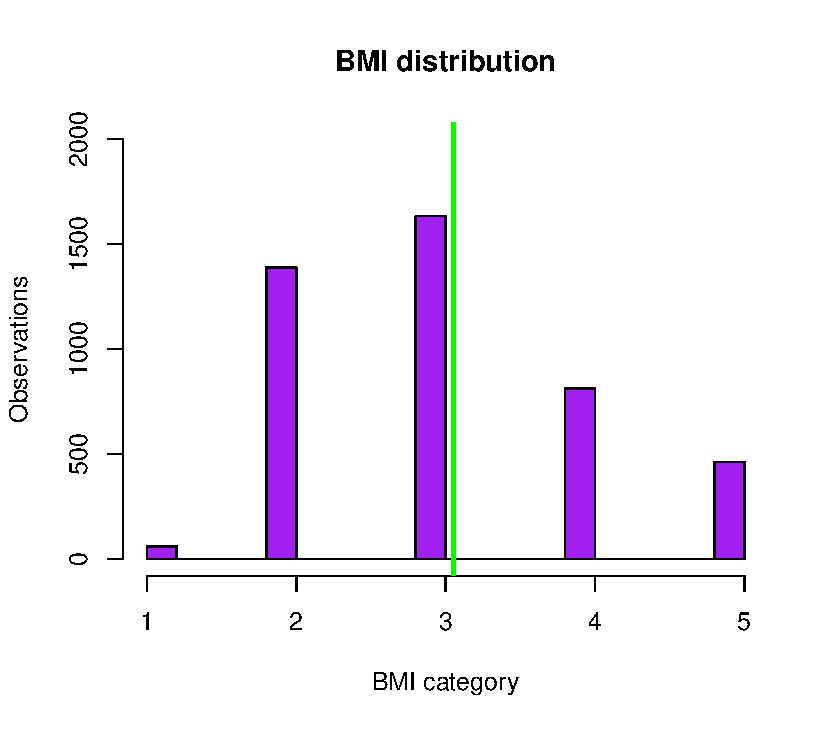
\includegraphics[width=0.75\linewidth]{rplots/RplotOverallDist.pdf}
		\caption{}
	\end{figure}
\end{frame}
\section{Analysis}
%------------------------------------------------
\begin{frame}{BMI Distribution (Med Takers)}\subsection{Med \& NonMed}
	\begin{figure}
		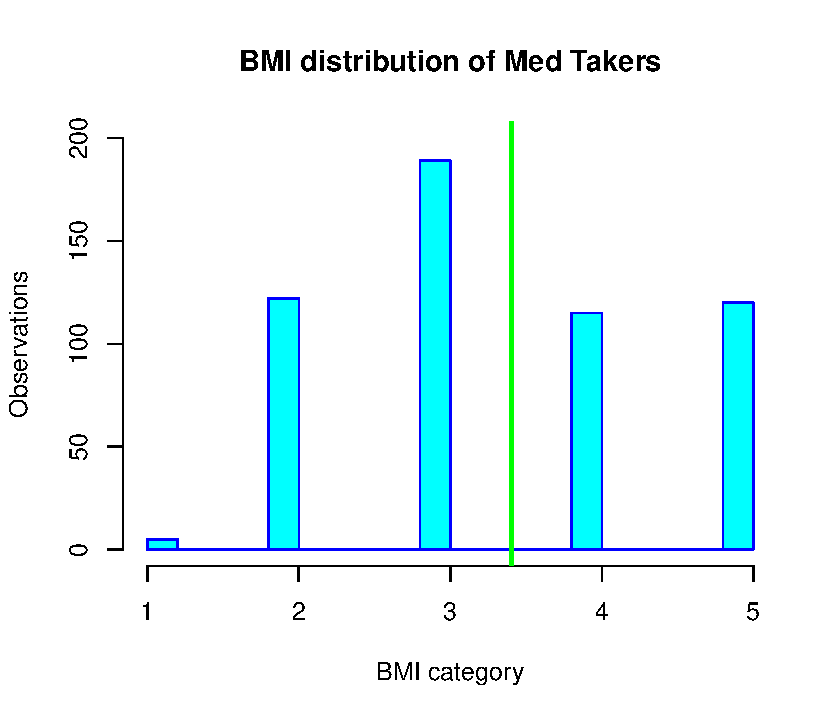
\includegraphics[width=0.75\linewidth]{rplots/Rplot.pdf}
		\caption{Figure One}
	\end{figure}
\end{frame}

\begin{frame}{BMI Distribution (Non-Med Takers)}
	\begin{figure}
		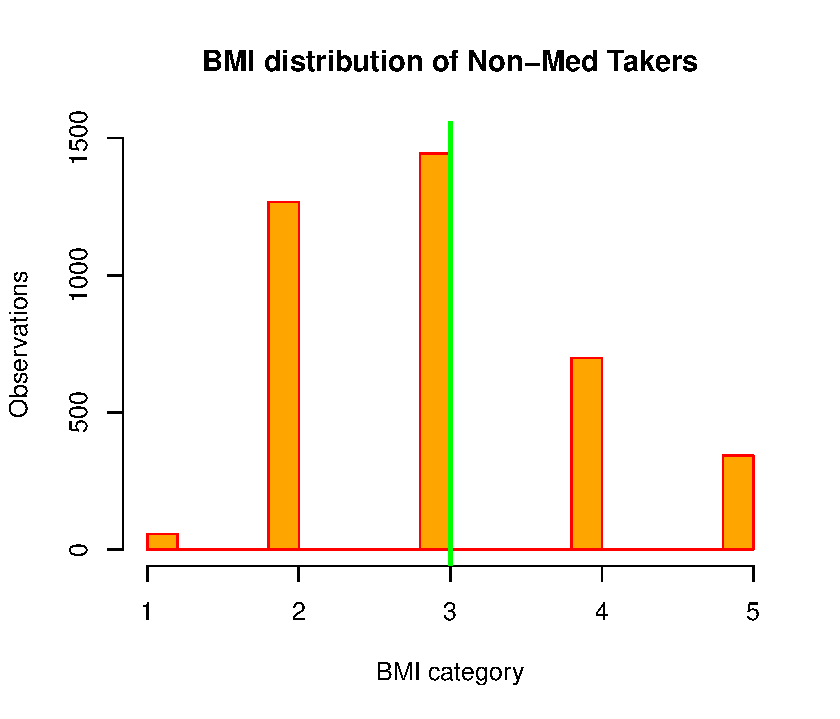
\includegraphics[width=0.75\linewidth]{rplots/Rplot01.pdf}
		\caption{Figure Two}
	\end{figure}
\end{frame}

\begin{frame}{Significance of BMI difference}
    \begin{itemize}
			\item We assume:
   \begin{itemize}
       \item Normality (CLT)
       \item Unknown, equal population variance
   \end{itemize}

   \item Hypotheses for t-test:
   \begin{equation}
    \begin{split} \label{hypothesis}
        H_0 :	\mu_{\text{MED}}-\mu_{\text{NoMED}} = 0 \\
        H_1 :	\mu_{\text{MED}}-\mu_{\text{NoMED}} > 0
    \end{split}
    \end{equation}
                \item Results:
                \begin{itemize}
       \item P Value=$10^{-20}$, We reject $H_0$. \\
       \item The difference of BMI between people who do not take mental health medications and those who do is statistically significant.
   \end{itemize}
			
		\end{itemize}
\end{frame}

\begin{frame}
	\frametitle{Male vs Female Tests} \subsection{Male \& Female} % Slide title, remove this command for no title
Analysing the effect of mental health medication interested us for the following reasons:	
    \begin{itemize}
        \item With the differences in male vs female hormonal systems, it was of interest how they affect both genders differently
        \item Existing sources, such as the Gates (2016) article state that women with prescribed medications gained more weight than men, and interested us into testing the means for both groups
    \end{itemize}
\end{frame}

\begin{frame}{BMI Distribution (Male Med Takers)}
	\begin{figure}
		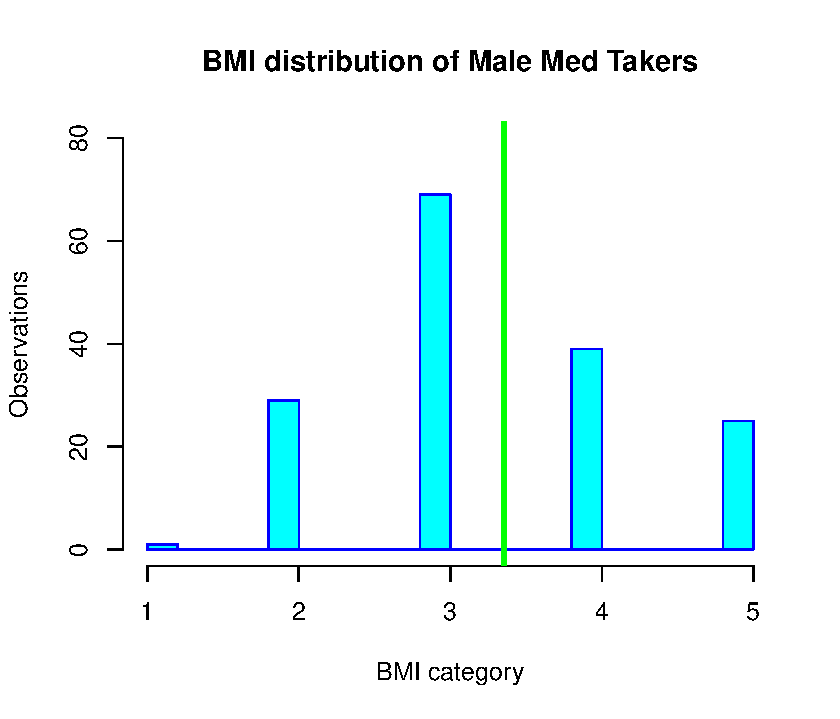
\includegraphics[width=0.75\linewidth]{rplots/Rplot02.pdf}
		\caption{}
	\end{figure}
\end{frame}

\begin{frame}{BMI Distribution (Male Non-Med Takers)}
	\begin{figure}
		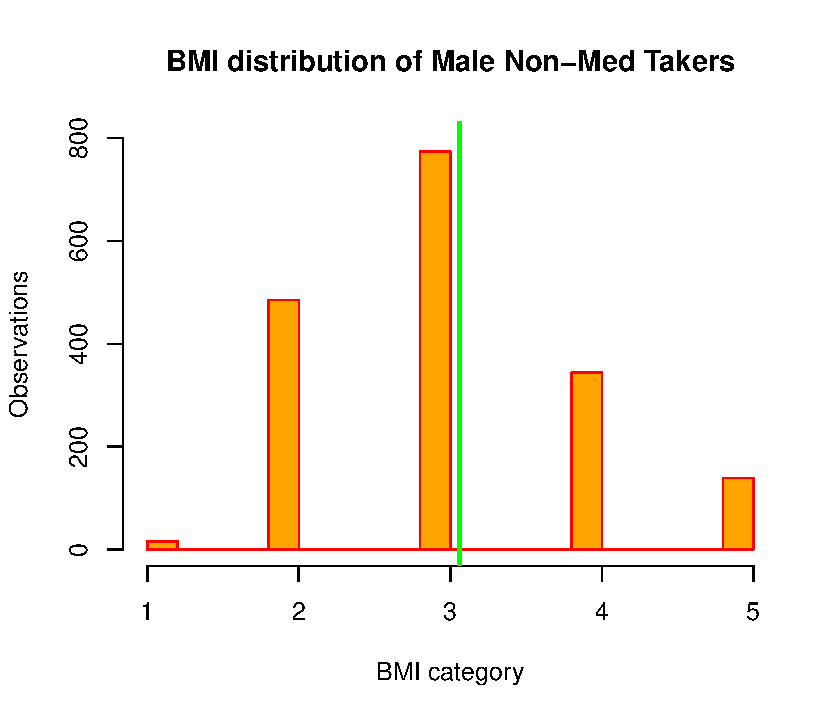
\includegraphics[width=0.75\linewidth]{rplots/Rplot03.pdf}
		\caption{}
	\end{figure}
\end{frame}


\begin{frame}{BMI Distribution (Female Med Takers)}
	\begin{figure}
		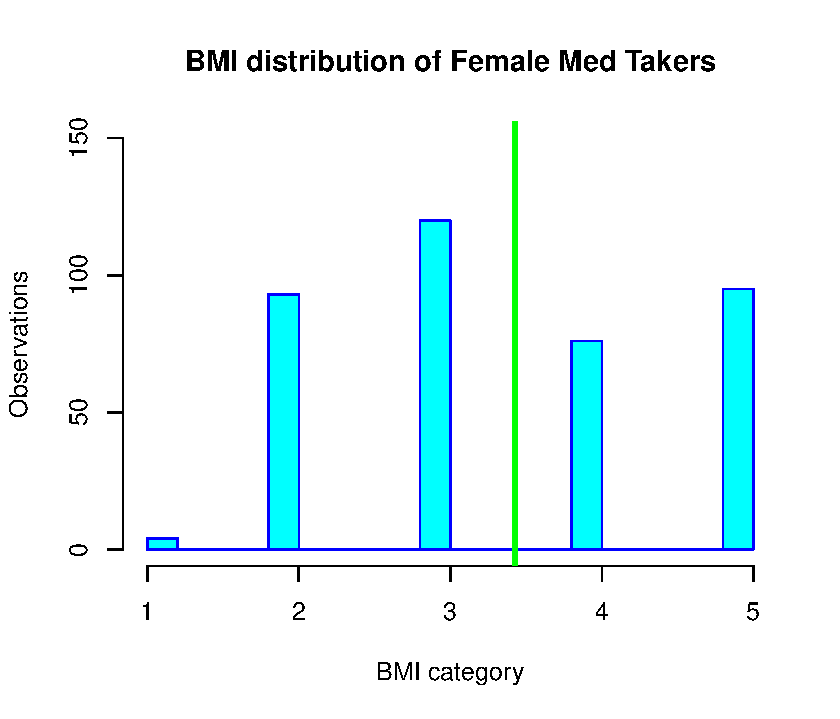
\includegraphics[width=0.75\linewidth]{rplots/Rplot04.pdf}
		\caption{}
	\end{figure}
\end{frame}


\begin{frame}{BMI Distribution (Female Non-Med Takers)}
	\begin{figure}
		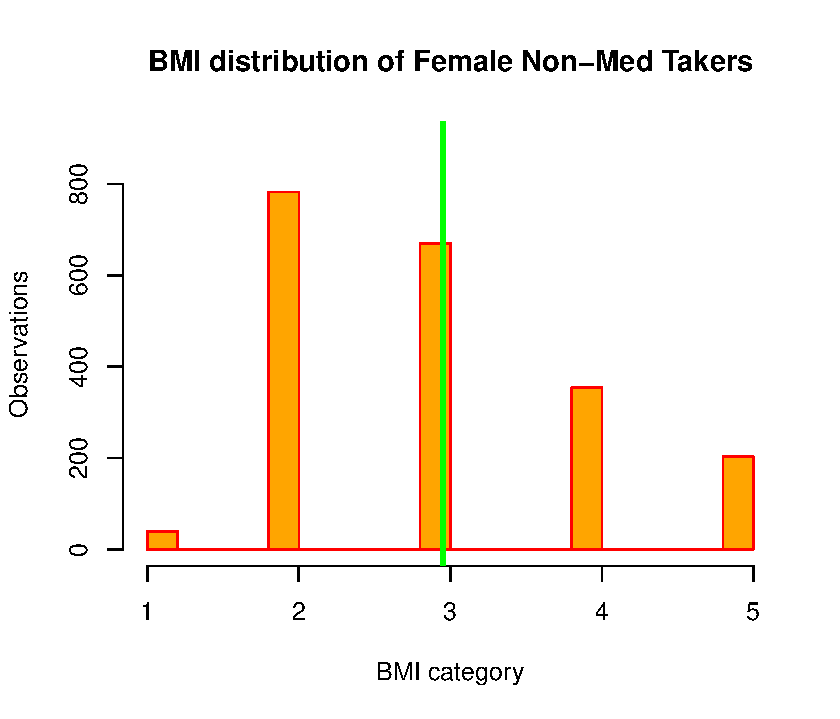
\includegraphics[width=0.75\linewidth]{rplots/Rplot05.pdf}
		\caption{}
	\end{figure}
\end{frame}

\begin{frame}{Significance of BMI difference}
    \begin{itemize}
			\item We assume:
   \begin{itemize}
       \item Normality (CLT)
       \item Unknown, equal population variance
   \end{itemize}

   \item Hypotheses for t-test:
  \begin{equation}
    \begin{split}
        H_0 :	\mu_{\text{MaleMED}}-\mu_{\text{FemaleMED}} = 0 \\
        H_1 :	\mu_{\text{MaleMED}}-\mu_{\text{FemaleMED}} \neq 0
    \end{split}
    \end{equation}\\
                \item Results:
                \begin{itemize}
       \item P Value=$0.26$, We fail to reject $H_0$. \\
       \item The difference of BMI between male and female who take mental health medication is not statistically significant.
   \end{itemize}
			
		\end{itemize}
\end{frame}

\begin{frame}
	\frametitle{Differences in Mental Heath Medicines}\subsection{Type of Medication} % Slide title, remove this command for no title

 Antipsychotics seem to cause more weight gain \citep{alonso,Gates2016,mahli,mazereel2020}.
 Mental health medicine are split in 3 categories, we decided to look at them individually:	
 \begin{itemize}
			\item Individuals prescribed only with antipsychotics 
			\item Individuals prescribed only with hypnotics
            \item Individuals prescribed only with antidepressants
		\end{itemize}
   
    
    
         This allowed us to look at independent samples and compare the general impact of these drugs, showing us which ones affected BMI the most
    
\end{frame}


\begin{frame}{BMI Distribution (Antidepressant Users)}
	\begin{figure}
		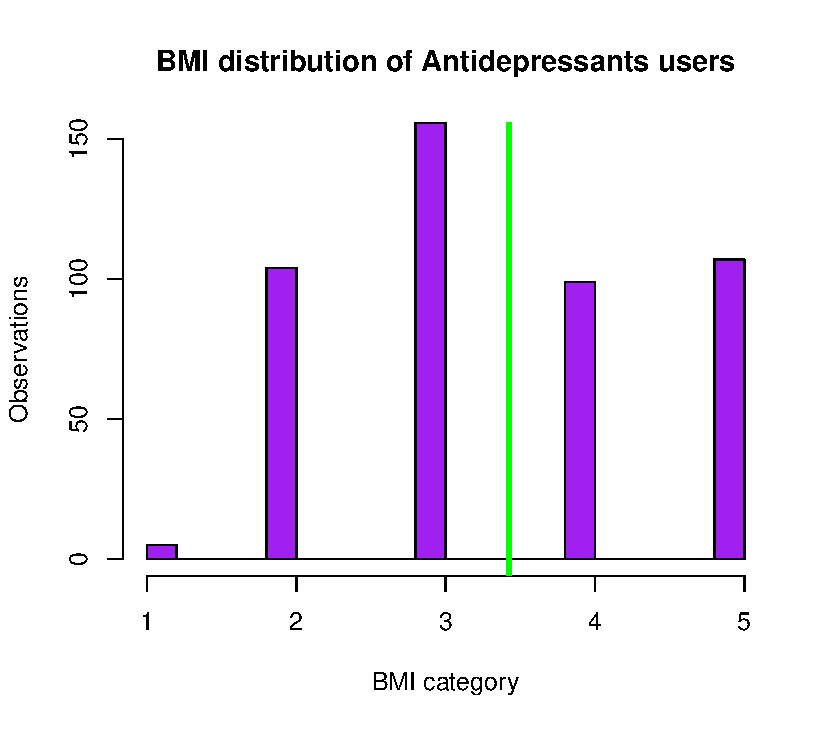
\includegraphics[width=0.75\linewidth]{rplots/RplotAntiDep.pdf}
		\caption{}
	\end{figure}
\end{frame}


\begin{frame}{BMI Distribution (Antipsychotics Users)}
	\begin{figure}
		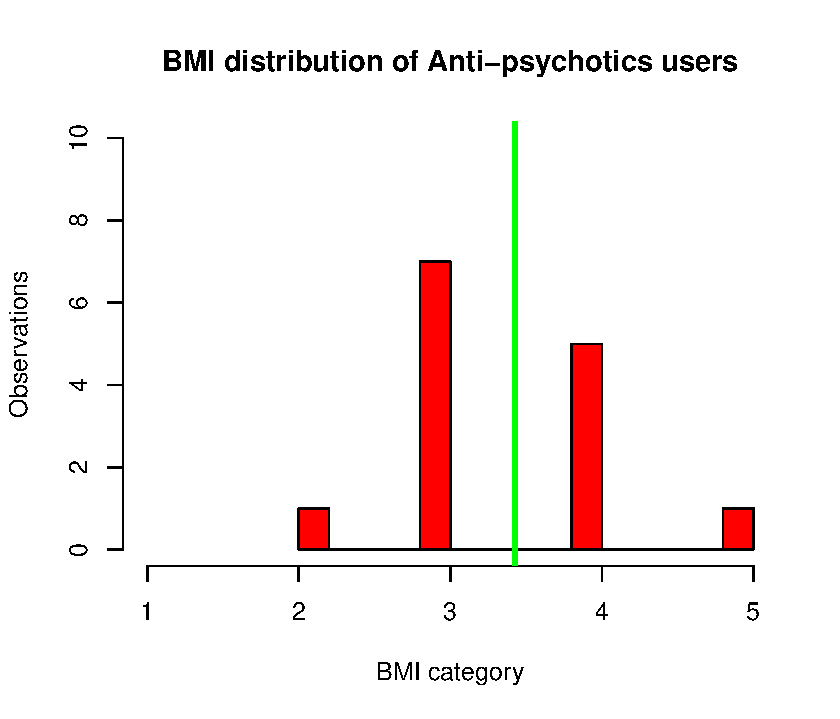
\includegraphics[width=0.75\linewidth]{rplots/Rplot07.pdf}
		\caption{}
	\end{figure}
\end{frame}



\begin{frame}{BMI Distribution (Hypnotics Users)}
	\begin{figure}
		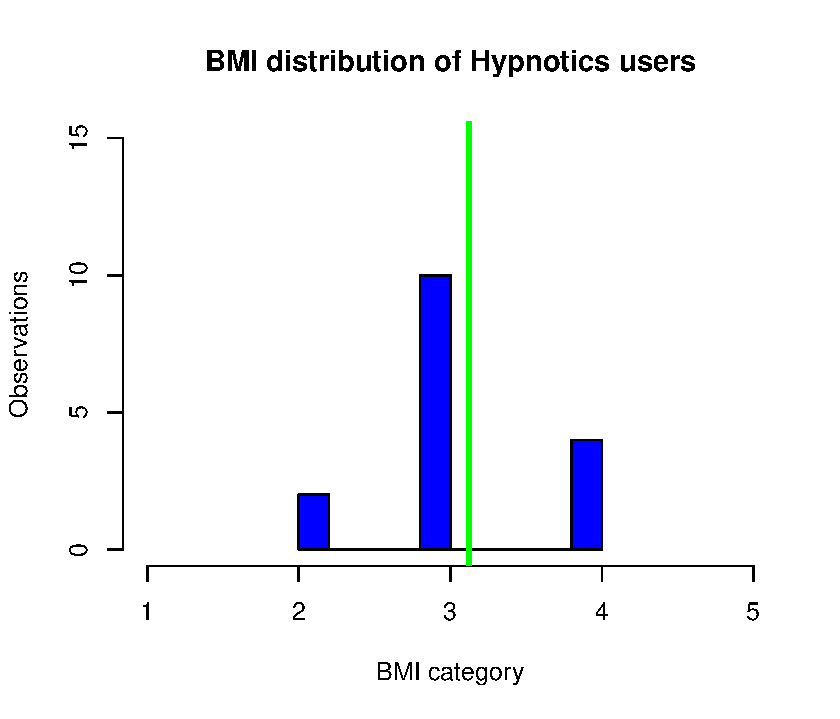
\includegraphics[width=0.75\linewidth]{rplots/Rplot08.pdf}
		\caption{}
	\end{figure}
\end{frame}

\begin{frame}{Significance of BMI difference}
    \begin{itemize}

   \item Hypotheses for Mann-Whitney U-tests:
  \begin{equation} 
    \begin{split}
        \label{mann_whitney_deppsy}
            H_0 :	\eta_{\text{Dep}} -\eta_{\text{Psy}} = 0 \\
            H_1 :	\eta_{\text{Dep}} - \eta_{\text{Psy}} < 0
    \end{split}
\end{equation}
\begin{equation}
    \begin{split}
     \label{mann_whitney_dephypno}
       H_0 :	\eta_{\text{Dep}}-\eta_{\text{Hypno}} = 0 \\
       H_1 :	\eta_{\text{Dep}}-\mu_{\text{Hypno}} \neq 0
    \end{split}
\end{equation}
\begin{equation} 
\begin{split}
\label{mann_whitney_psyhypno}
        H_0 :	\eta_{\text{Psy}}-\eta_{\text{Hypno}} = 0 \\
        H_1 :	\eta_{\text{Psy}}-\mu_{\text{Hypno}} > 0
        \end{split}
 \end{equation} \\
                \item Results:
                \begin{itemize}
       \item P Value=$0.45$, $0.32$, $0.14$, We fail to reject all $H_0$. \\
       \item The difference of BMI between different mental health medications is not statistically significant.
   \end{itemize}
			
		\end{itemize}
\end{frame}

%------------------------------------------------



%------------------------------------------------


%------------------------------------------------



%----------------------------------------------------------------------------------------
%	CLOSING SLIDE
%----------------------------------------------------------------------------------------

\begin{frame} \section{Conclusion}
	\frametitle{Conclusion}\subsection{Results} % Slide title, remove this command for no title
 After our analysis, we have come to conclude:	
    \begin{itemize}
        \item Mental Health medications may increase a person's BMI.
        \item Mental health medications may not affect men and women differently.
        \item Different types of mental health medications may not differently impact BMI.
    \end{itemize}
\end{frame}

%----------------------------------------------------------------------------------------
%	ACKNOWLEDGMENTS SLIDE
%----------------------------------------------------------------------------------------

\begin{frame}
	\frametitle{Acknowledgements}\subsection{Acknowledgements} % Slide title, remove this command for no title
We extend our heartfelt gratitude to:
    \begin{itemize}
        \item Prof. Jeremy Smith for his support throughout the project
        \item Open source community for resources available
        \item University of Warwick for resources provided
    \end{itemize}

\end{frame}


\begin{frame} % The optional argument 'plain' hides the headline and footline
    \frametitle{References}\subsection{References}

\def\bibfont{\tiny}
 \bibliographystyle{agsm}
\bibliography{ref}
		
\end{frame}

%----------------------------------------------------------------------------------------

\end{document} 